


\section{Descripción General del Desarrollo del Protocolo}
El protocolo criptográfico para evitar duplicados almacenados en la nube, es un proyecto que involucra la tecnología de software para ofrecer un funcionamiento eficiente y útil para las necesidades de los usuarios que se encuentran inmersos en el cómputo nube. 
Nuestro protocolo, se compone a su vez de diferentes módulos. Cada uno de ellos busca satisfacer: \\ 

\begin{itemize}

\item La seguridad de los archivos de los usuarios en la nube
\item Almacenamiento seguro en la sube
\item Conexión de diversos usuarios 
\item Ahorro en el consumo de espacio ofrecido en la nube 
\item Fácil acceso al almacenamiento de los archivos de los usuarios 

\end{itemize} 

Para lograrlo, el protocolo criptográfico se compone de diversos módulos que a su vez integran diferentes aplicaciones criptográficas. Dichos módulos serán detallados en las próximas secciones. 

\section{Aplicación Criptográfica (Cifrado / Descifrado)}

Éste módulo del protocolo es de suma importancia para ofrecer la seguridad de los archivos como se menciona anteriormente, ya que en éste módulo se lleva a cabo para blindar un archivo, es decir cifrarlo.  En este módulo participan: 

	\begin{itemize}
	\item El archivo que se almacenará en la nube.
	\item La clave para poder cifrarlo, que en este caso es la llave \textit{(z)} generada por el cliente en el módulo anterior. 
	\end{itemize}
El desarrollo de éste módulo, fue realizado como el módulo anterior en el lenguaje de programación Python versión 2.7.3. Además de que para la implementación del algoritmo de cifrado AES se utilizó principalmente la biblioteca criptográfica Pycripto 2.3. 

\subsection{Cifrado}
Éste algoritmo que forma parte de la aplicación criptográfica, se lleva a cabo del lado del cliente, dicho algoritmo de cifrado se encargará de brindar la seguridad a los archivos que los usuarios deseen almacenar en la nube. \\
El cifrado de archivos se lleva a cabo bajo la utilización del algoritmo de cifrado \textbf{AES} que proveé la librería criptográfica \textbf{PyCripto 2.3} propia del lenguaje \textbf{Python}. Ésta libreria poseé la seguridad necesaria para satisfacer a los requerimientos del protocolo criptográfico.  \\ 
La implementación del algoritmo, se llevó a cabo de la siguiente manera: 

	\begin{itemize}
		\item Las librerías utilizadas para llevar a cabo el cifrado de archivos son las siguientes
			\begin{figure}[H]
			\centering
			\includegraphics[width=10cm, height=1.5cm]{./images/cifrado/01.jpg}
			\caption{Librerías de Python (Cifrado)}
			\label{fig:6-2-1} 
			\end{figure} 
		Siendo \textbf{haslib, Crypto.Cipher.AES, Crypto.Util.Counter, hmac} librerías criptográficas, es decir, utilizadas para llevar a cabo operaciones relacionadas con la implementación del algoritmo de cifrado \textit{AES} en sus 3 tipos de tamaños de claves \textit{(128, 192, 256 bits)}.\\ \\ 
La librería \textbf{tkFileDialog} utilizada para cuando el usuario desee elegir desde su PC un archivo para almacenarlo en la nube, se abra un panel de archivos, permitiendo acceder a sus carpetas personales, y de manera gráfica, dicho usuario pueda elegir el archivo con solo darle un clic. \\ \\ 
\textbf{Base 64} Una librería utilizada para convertir las salidas del algoritmo \textit{AES} a caracteres dentro del \textit{código ASCII}, ya que \textit{AES} involucra funciones que obtienen a la salida caracteres en el sistema hexadecimal y son difíciles de procesar en su forma original para su uso posterior. 


		\item Para poder comenzar el proceso de cifrado, es necesario obtener la clave que se utilizará para llevar a cabo el proceso. \\ Dicha clave se obtiene de la siguiente manera: 
			\begin{figure}[H]
			\centering
			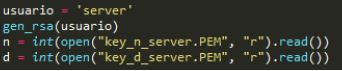
\includegraphics[width=10cm, height=1cm]{./images/cifrado/02.jpg}
			\caption{Obtención de Clave de Cifrado}
			\label{fig:6-2-2} 
			\end{figure} 
	Abrimos el archivo \textbf{key\_z} y almacenamos su contenido en la variable \textbf{contentK}. Éste archivo contiene la clave que se necesita para poder cifrar el archivo que el usuario desea, dicha \textit{clave (z)} fue generada y escrita en este archivo en el módulo anterior. 

		\item Se crea un objeto de tipo \textit{AES} que almacenamos en la variable \textbf{cipher}, el cual contiene como parámetros la clave que obtuvo del archivo  \textbf{key\_z}, el modo de operación que se utilizará \textbf{(CTR)}, etc.
			\begin{figure}[H]
			\centering
			\includegraphics[width=15cm, height=1cm]{./images/cifrado/03.jpg}
			\caption{Objeto de Tipo AES}
			\label{fig:6-2-3} 
			\end{figure} 

		\item Para cifrar el archivo, mandamos llamar al método \textbf{\textit{encrypt(m)}} \textit{(m almacena el contenido del archivo que se desea cifrar)} y almacenamos el resultado de dicho método en la variable \textbf{ctext.}
			\begin{figure}[H]
			\centering
			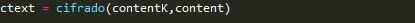
\includegraphics[width=10cm, height=1cm]{./images/cifrado/04.jpg}
			\caption{Método Encrypt}
			\label{fig:6-2-4} 
			\end{figure} 

		\item Para finalizar, mandamos escribir a un archivo temporal el cifrado que obtuvimos en la variable \textbf{ctext.}
			\begin{figure}[H]
			\centering
			\includegraphics[width=13cm, height=1.5cm]{./images/cifrado/05.jpg}
			\caption{Escribir Cifrado en Archivo Temporal}
			\label{fig:6-2-4} 
			\end{figure} 


	\end{itemize}


\subsection{Descifrado}
Éste algoritmo que forma parte de la aplicación criptográfica, al igual que el cifrado, se lleva a cabo del lado del cliente, éste algoritmo será el encargado de que los usuarios puedan recuperar sus archivos originales, es decir, tomar de la nube aquel archivo que se encuentre cifrado y posteriormente descifrarlo para poder acceder a este archivo en su forma original. \\
El descifrado de archivos se lleva a cabo bajo la utilización del algoritmo de descifrado \textbf{AES} que, al igual que el cifrado lo proveé la librería criptográfica \textbf{PyCripto 2.3} propia del lenguaje \textbf{Python}.   \\ 
La implementación del algoritmo, se llevó a cabo de la siguiente manera: 

\begin{itemize}
	\item Las librerías utilizadas para llevar a cabo el descifrado de archivos son las siguientes: 
			\begin{figure}[H]
			\centering
			\includegraphics[width=8.5cm, height=1cm]{./images/descifrado/01.jpg}
			\caption{Librerías de Python (Descifrado)}
			\label{fig:6-3-1} 
			\end{figure} 
Siendo \textbf{Crypto.Cipher.AES, Crypto.Util.Counter}, librerías criptográficas, es decir, utilizadas para llevar a cabo operaciones relacionadas con la implementación del algoritmo de descifrado \textit{AES} en sus 3 tipos de tamaños de claves \textit{(128, 192, 256 bits)}. 

	\item Al igual que en el proceso de cifrado, para comenzar dicho proceso es necesario obtener la clave que se utilizará para el descifrado. Dicha clave se obtiene de la siguiente manera:  

			\begin{figure}[H]
			\centering
			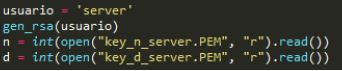
\includegraphics[width=10cm, height=1cm]{./images/cifrado/02.jpg}
			\caption{Obtención de Clave de Descifrado}
			\label{fig:6-3-2} 
			\end{figure} 

Abrimos el archivo \textbf{key\_z} y almacenamos su contenido en la variable \textbf{contentK}. 

		\item El siguiente paso, es abrir el archivo temporal que se generó al momento de cifrar el archivo del usuario. 
			\begin{figure}[H]
			\centering
			\includegraphics[width=10cm, height=1cm]{./images/descifrado/03.jpg}
			\caption{Obtención del cifrado}
			\label{fig:6-3-3} 
			\end{figure} 

Una vez dentro del archivo, almacenamos el cifrado en la variable \textbf{textcifrado} para utilizarlo posteriormente. 

		\item Creamos un objeto \textit{AES} que almacenamos en la variable \textbf{ciphe}r, el cual contiene como parámetros la llave que obtuvo del archivo \textbf{key\_z }, el modo de operación que se utilizará para el descifrado\textbf{(CTR)}, etc.
			\begin{figure}[H]
			\centering
			\includegraphics[width=15cm, height=1cm]{./images/cifrado/03.jpg}
			\caption{Objeto de Tipo AES}
			\label{fig:6-3-4} 
			\end{figure} 


		\item Desciframos el archivo, mandamos llamar al método \textbf{\textit{decrypt(textcifrado)}}  y almacenamos el resultado de dicho método en la variable \textbf{plaintext}
			\begin{figure}[H]
			\centering
			\includegraphics[width=9cm, height=1cm]{./images/descifrado/05.jpg}
			\caption{Método Decrypt}
			\label{fig:6-3-5} 
			\end{figure} 

		\item Para finalizar, mandamos escribir a un archivo \textbf{fname} \textit{(Es el nombre del archivo original del usuario)} el archivo tal y como estaba antes de cifrarlo. 
			\begin{figure}[H]
			\centering
			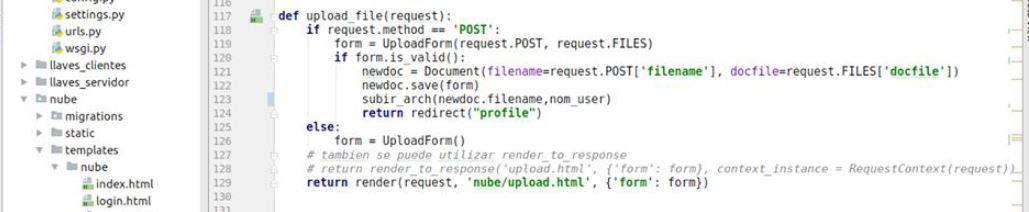
\includegraphics[width=10cm, height=1.5cm]{./images/descifrado/06.jpg}
			\caption{Escribir Archivo Original en la Ruta Inicial}
			\label{fig:6-3-6} 
			\end{figure} 

\end{itemize}





